\documentclass[tikz,border=10pt]{standalone}
\usepackage{tikz}
\usetikzlibrary{arrows.meta,positioning,fit,calc}

\begin{document}
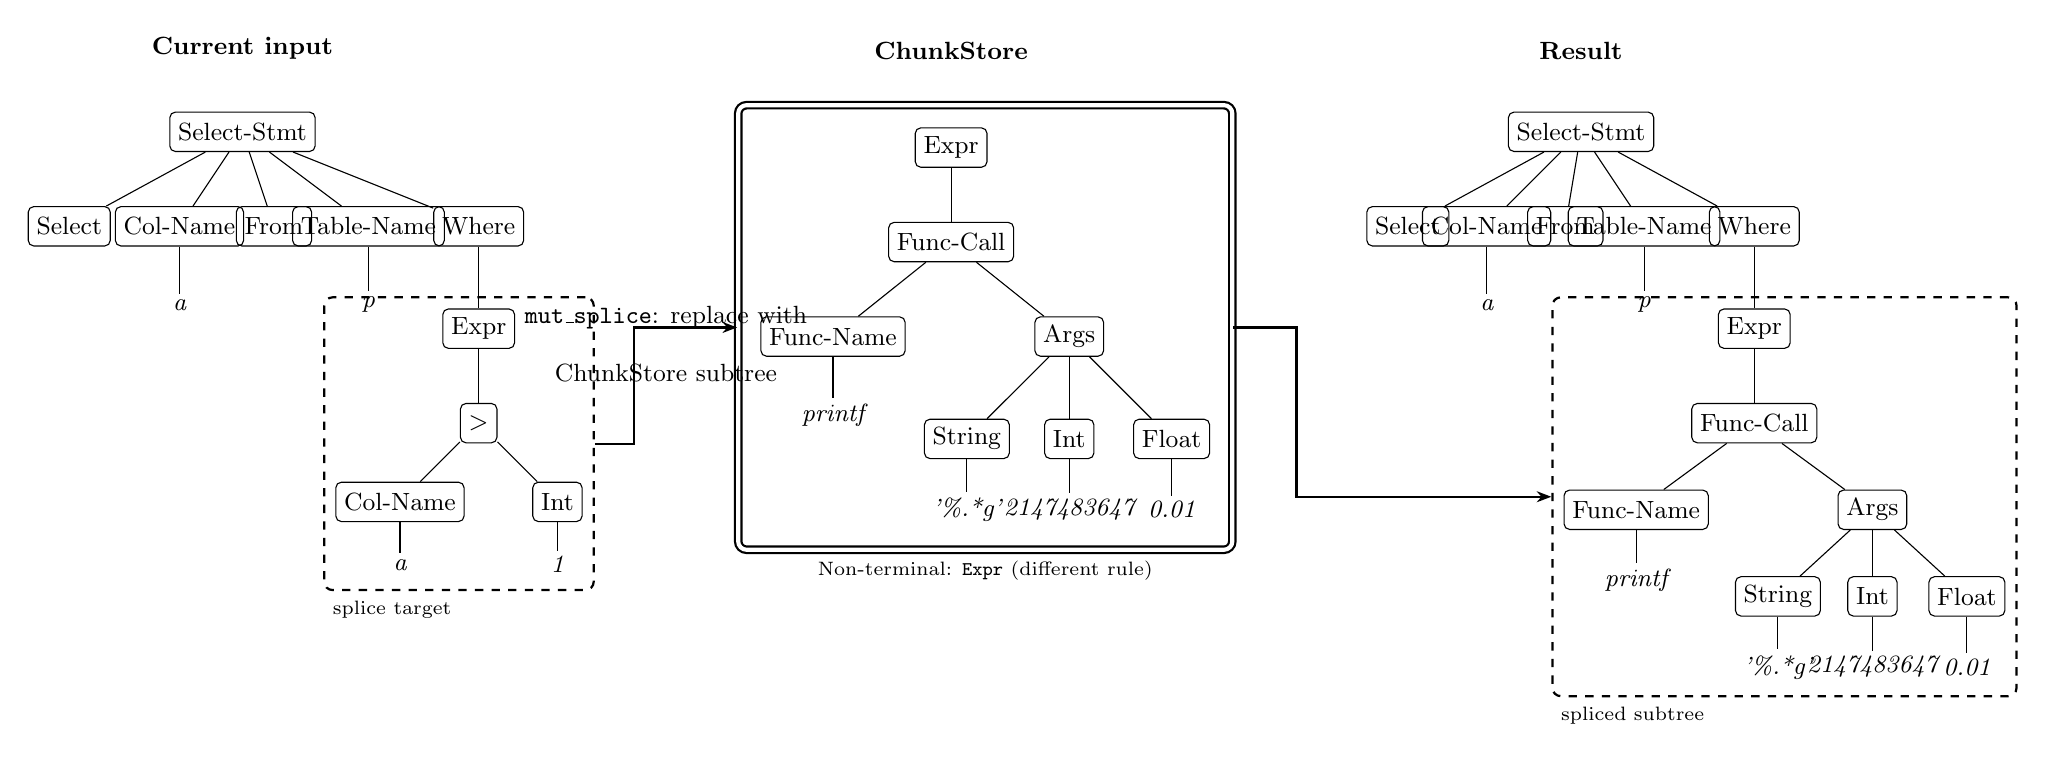
\begin{tikzpicture}[
    every node/.style={font=\small},
    % Non-terminals: rounded rectangles
    nt/.style={rectangle, rounded corners=2pt, draw, thin,
        inner sep=3pt, minimum height=0.5cm, font=\small},
    % Terminals: italic
    tm/.style={font=\small\itshape, inner sep=2pt},
    % Dashed highlight rectangle
    highlight/.style={draw, dashed, thick, rounded corners=3pt, inner sep=4pt},
    % ChunkStore box: double border
    chunkstore/.style={rectangle, draw, double, double distance=1.5pt,
        thick, rounded corners=3pt, inner sep=8pt},
    % Arrow style
    arr/.style={-{Stealth[scale=0.8]}, thick},
    % Section label
    seclabel/.style={font=\small\bfseries, anchor=south},
]

% ============================================================
% SECTION 1: Current input (left)
% Tree: Select-Stmt -> Select, Col-Name(a), From, Table-Name(p), Where, Expr(>)
% ============================================================
\node[seclabel] at (0, 4.8) {Current input};

\node[nt] (s1root) at (0, 4) {Select-Stmt};

\node[nt] (s1sel) at (-2.2, 2.8) {Select};
\node[nt] (s1col) at (-0.8, 2.8) {Col-Name};
\node[nt] (s1from) at (0.4, 2.8) {From};
\node[nt] (s1tbl) at (1.6, 2.8) {Table-Name};
\node[nt] (s1where) at (3.0, 2.8) {Where};
\node[nt] (s1expr) at (3.0, 1.5) {Expr};

\node[tm] (s1a) at (-0.8, 1.8) {a};
\node[tm] (s1p) at (1.6, 1.8) {p};

\node[nt] (s1gt) at (3.0, 0.3) {$>$};
\node[nt] (s1colr) at (2.0, -0.7) {Col-Name};
\node[nt] (s1int) at (4.0, -0.7) {Int};
\node[tm] (s1av) at (2.0, -1.5) {a};
\node[tm] (s1one) at (4.0, -1.5) {1};

% Edges section 1
\draw (s1root) -- (s1sel);
\draw (s1root) -- (s1col);
\draw (s1root) -- (s1from);
\draw (s1root) -- (s1tbl);
\draw (s1root) -- (s1where);
\draw (s1col) -- (s1a);
\draw (s1tbl) -- (s1p);
\draw (s1where) -- (s1expr);
\draw (s1expr) -- (s1gt);
\draw (s1gt) -- (s1colr);
\draw (s1gt) -- (s1int);
\draw (s1colr) -- (s1av);
\draw (s1int) -- (s1one);

% Dashed rectangle around Expr subtree (splice target)
\node[highlight, fit=(s1expr)(s1gt)(s1colr)(s1int)(s1av)(s1one)] (s1hl) {};
\node[font=\scriptsize, anchor=north west] at (s1hl.south west) {splice target};

% ============================================================
% SECTION 2: ChunkStore (center)
% ============================================================
\node[seclabel] at (9, 4.8) {ChunkStore};

% ChunkStore container
\node[nt] (csexpr) at (9, 3.8) {Expr};
\node[nt] (csfunc) at (9, 2.6) {Func-Call};
\node[nt] (csfname) at (7.5, 1.4) {Func-Name};
\node[nt] (csargs) at (10.5, 1.4) {Args};
\node[tm] (csprintf) at (7.5, 0.4) {printf};
\node[nt] (csfmt) at (9.2, 0.1) {String};
\node[nt] (csint) at (10.5, 0.1) {Int};
\node[nt] (csflt) at (11.8, 0.1) {Float};
\node[tm] (csfmtv) at (9.2, -0.8) {'\%.*g'};
\node[tm] (csintv) at (10.5, -0.8) {2147483647};
\node[tm] (csfltv) at (11.8, -0.8) {0.01};

% Edges section 2
\draw (csexpr) -- (csfunc);
\draw (csfunc) -- (csfname);
\draw (csfunc) -- (csargs);
\draw (csfname) -- (csprintf);
\draw (csargs) -- (csfmt);
\draw (csargs) -- (csint);
\draw (csargs) -- (csflt);
\draw (csfmt) -- (csfmtv);
\draw (csint) -- (csintv);
\draw (csflt) -- (csfltv);

% ChunkStore double-border box
\node[chunkstore, fit=(csexpr)(csfunc)(csfname)(csargs)(csprintf)(csfmt)(csint)(csflt)(csfmtv)(csintv)(csfltv)] (csbox) {};

% Label below
\node[font=\scriptsize, anchor=north] at (csbox.south) {Non-terminal: \texttt{Expr} (different rule)};

% ============================================================
% SECTION 3: Result (right)
% Tree: SELECT a FROM p WHERE printf('%.*g', 2147483647, 0.01)
% ============================================================
\node[seclabel] at (17, 4.8) {Result};

\node[nt] (r1root) at (17, 4) {Select-Stmt};

\node[nt] (r1sel) at (14.8, 2.8) {Select};
\node[nt] (r1col) at (15.8, 2.8) {Col-Name};
\node[nt] (r1from) at (16.8, 2.8) {From};
\node[nt] (r1tbl) at (17.8, 2.8) {Table-Name};
\node[nt] (r1where) at (19.2, 2.8) {Where};

\node[tm] (r1a) at (15.8, 1.8) {a};
\node[tm] (r1p) at (17.8, 1.8) {p};

% Spliced-in Expr subtree
\node[nt] (r1expr) at (19.2, 1.5) {Expr};
\node[nt] (r1func) at (19.2, 0.3) {Func-Call};
\node[nt] (r1fname) at (17.7, -0.8) {Func-Name};
\node[nt] (r1args) at (20.7, -0.8) {Args};
\node[tm] (r1printf) at (17.7, -1.7) {printf};
\node[nt] (r1fmt) at (19.5, -1.9) {String};
\node[nt] (r1int) at (20.7, -1.9) {Int};
\node[nt] (r1flt) at (21.9, -1.9) {Float};
\node[tm] (r1fmtv) at (19.5, -2.8) {'\%.*g'};
\node[tm] (r1intv) at (20.7, -2.8) {2147483647};
\node[tm] (r1fltv) at (21.9, -2.8) {0.01};

% Edges section 3
\draw (r1root) -- (r1sel);
\draw (r1root) -- (r1col);
\draw (r1root) -- (r1from);
\draw (r1root) -- (r1tbl);
\draw (r1root) -- (r1where);
\draw (r1col) -- (r1a);
\draw (r1tbl) -- (r1p);
\draw (r1where) -- (r1expr);
\draw (r1expr) -- (r1func);
\draw (r1func) -- (r1fname);
\draw (r1func) -- (r1args);
\draw (r1fname) -- (r1printf);
\draw (r1args) -- (r1fmt);
\draw (r1args) -- (r1int);
\draw (r1args) -- (r1flt);
\draw (r1fmt) -- (r1fmtv);
\draw (r1int) -- (r1intv);
\draw (r1flt) -- (r1fltv);

% Dashed rectangle around the spliced-in Expr subtree
\node[highlight, fit=(r1expr)(r1func)(r1fname)(r1args)(r1printf)(r1fmt)(r1int)(r1flt)(r1fmtv)(r1intv)(r1fltv)] (r1hl) {};
\node[font=\scriptsize, anchor=north west] at (r1hl.south west) {spliced subtree};

% ============================================================
% ARROWS between sections
% ============================================================

% Arrow from ChunkStore to the result (showing insertion)
\draw[arr] (csbox.east) -- ++(0.8,0) |- (r1hl.west);

% Arrow from Section 1 highlight to ChunkStore (showing replacement)
\draw[arr] (s1hl.east) -- ++(0.5,0) |- (csbox.west);

% Operation label
\node[font=\small, align=center, anchor=south] at ($(s1hl.east)!0.5!(csbox.west) + (0, 0.6)$)
    {\texttt{mut\_splice}: replace with};
\node[font=\small, align=center, anchor=north] at ($(s1hl.east)!0.5!(csbox.west) + (0, 0.4)$)
    {ChunkStore subtree};

\end{tikzpicture}
\end{document}
